\documentclass[10pt,fleqn, twocolumn]{IEEEtran}
\usepackage{amsfonts}
\usepackage{amsthm}
\usepackage{amsmath}
\usepackage{graphicx}
\usepackage{fancyhdr}


\newtheorem{Prop}{Proposition}
\newtheorem{lemma}{Lemma}
\newtheorem{theorem}{Theorem}

\setlength{\parindent}{3em} \setlength{\oddsidemargin}{0in}
\setlength{\textwidth}{6.5in} % sets 1in left and right margins
\setlength{\topmargin}{0.20in} % change to 0.2in for regular latex
%\setlength{\headheight}{0in}
%\setlength{\footheight}{0.5in}
\setlength{\footskip}{0.5in}
\setlength{\textheight}{9.0in} %sets 1in top and bottom margins
\renewcommand{\baselinestretch}{1} %set to 1.5 for double spacing.

\newcommand{\br}{{\mathbf r}}
\newcommand{\bA}{{\mathbf A}}
\newcommand{\ba}{{\bf a}}
\newcommand{\bb}{{\bf b}}
\newcommand{\bc}{{\bf c}}
\newcommand{\bC}{{\bf C}}
\newcommand{\bd}{{\bf d}}
\newcommand{\be}{{\bf e}}
\newcommand{\bE}{{\bf E}}
\newcommand{\bbf}{{\bf f}}
\newcommand{\bF}{{\bf F}}
\newcommand{\bh}{{\bf h}}
\newcommand{\bH}{{\bf H}}
\newcommand{\bg}{{\bf g}}
\newcommand{\bG}{{\bf G}}
\newcommand{\bq}{{\bf q}}
\newcommand{\bs}{{\bf s}}
\newcommand{\bm}{{\bf m}}
\newcommand{\bn}{{\bf n}}
\newcommand{\bu}{{\bf u}}
\newcommand{\bv}{{\bf v}}
\newcommand{\bw}{{\bf w}}
\newcommand{\bx}{{\bf x}}
\newcommand{\by}{{\bf y}}
\newcommand{\bz}{{\bf z}}
\newcommand{\bL}{{\bf L}}
\newcommand{\bM}{{\bf M}}
\newcommand{\bN}{{\bf N}}
\newcommand{\bS}{{\bf S}}
\newcommand{\bT}{{\bf T}}
\newcommand{\bD}{{\bf D}}
\newcommand{\bX}{{\bf X}}
\newcommand{\bP}{{\bf P}}
\newcommand{\bQ}{{\bf Q}}
\newcommand{\bI}{{\bf I}}
\newcommand{\bR}{{\bf R}}
\newcommand{\bU}{{\bf U}}
\newcommand{\bV}{{\bf V}}
\newcommand{\bW}{{\bf W}}
\newcommand{\bY}{{\bf Y}}
\newcommand{\bZ}{{\bf Z}}
\newcommand{\bJ}{{\bf J}}
\newcommand{\bB}{{\bf B}}
\newcommand{\bzero}{{\bf 0}}
\newcommand{\bgamma}{{\mbox {\boldmath $\gamma$}}}
\newcommand{\btheta}{{\mbox {\boldmath $\theta$}}}
\newcommand{\bvartheta}{{\mbox {\boldmath $\vartheta$}}}
\newcommand{\bDelta}{{\mbox {\boldmath $\Delta$}}}
\newcommand{\bLambda}{{\mbox {\boldmath $\Lambda$}}}
\newcommand{\bPsi}{{\mbox {\boldmath $\Psi$}}}
\newcommand{\bPhi}{{\mbox {\boldmath $\Phi$}}}
\newcommand{\bcA}{{\mbox {\boldmath ${\cal A}$}}}
\newcommand{\bcB}{{\mbox {\boldmath ${\cal B}$}}}
\newcommand{\bcC}{{\mbox {\boldmath ${\cal C}$}}}
\newcommand{\bcD}{{\mbox {\boldmath ${\cal D}$}}}
\newcommand{\bcF}{{\mbox {\boldmath ${\cal F}$}}}
\newcommand{\bcG}{{\mbox {\boldmath ${\cal G}$}}}
\newcommand{\bcL}{{\mbox {\boldmath ${\cal L}$}}}
\newcommand{\bcN}{{\mbox {\boldmath ${\cal N}$}}}
\newcommand{\bcR}{{\mbox {\boldmath ${\cal R}$}}}
\newcommand{\bcS}{{\mbox {\boldmath ${\cal S}$}}}
\newcommand{\bcH}{{\mbox {\boldmath ${\cal H}$}}}
\newcommand{\bcI}{{\mbox {\boldmath ${\cal I}$}}}
\newcommand{\bcO}{{\mbox {\boldmath ${\cal O}$}}}
\newcommand{\bcP}{{\mbox {\boldmath ${\cal P}$}}}
\newcommand{\bcQ}{{\mbox {\boldmath ${\cal Q}$}}}
\newcommand{\bcV}{{\mbox {\boldmath ${\cal V}$}}}
\newcommand{\bcW}{{\mbox {\boldmath ${\cal W}$}}}


\title{Optimizing Hierarchical Modulation}
\author{\\LG Electronics Mobile Research\\San Diego, CA 92131-1807}
\date{}
\begin{document}
\maketitle
\begin{abstract}\small
One enhanced hierarchical modulation and three optimizationn
schemes for it are presented and analyzed in this paper. The
enhanced hierarchical modulation is to rotate the
enhancement-layer signal constellation(s) for better performance.
The first optimization scheme is to optimize the enhancement-layer
signal constellation(s) for higher spectral efficiency. The second
scheme is to maximize the modulation efficiency for lower
bit-error rate. The last one is to control the
peak-to-average-power ratio for higher amplifier power efficiency,
especially for multicarrier applications. All proposed schemes are
simple and efficient. They can be used to recover the performane
loss in regular hierarchical modulations with little complexity
increase. Computer simulations are provided to support our
conclusions.
\end{abstract}

\section{Introduction}
Broadcast multicast service (BCMCS) has increasingly been popular
for delivering multimedia content to mobile users. BCMCS can be
offered through either a 3rd generation and beyond radio access
network like WCDMA or cdma2000 network or a dedicate digital
broadcast infrastructure like DVB-T/H/S2, MediaFLO, DMB, etc. Most
of them employ OFDM air interface due to its high spectral
efficiency with simple receiver design. Traditional digital
broadcast system is designed with the tradeoff between maximum
achievable rate and intended coverage in mind. Their capacities
are limited by maximum transmit power and worst channel conditions
so that every user in the intended coverage area can reliably
receive services. The users under good reception condition and
with a advanced receiver may not have many advantages, even though
their achievable throughput can be much higher.

Recently there are lots of interests in upgrading existing digital
broadcast systems with more services for new users while keep
existing users unchanged, delivering  additional or better quality
of service (QoS) to users with advanced receivers while still
guaranteing others' services, and providing unequal protection on
digital contents~\cite{DVB,MediaFLO,Jiang05,UMB}. Many
technologies are under investigation for these goals, e.g.,
rateless coding, hierarchical modulation, multiple-input
multiple-output (MIMO) and selective retransmission. Right now,
backward compatibility is one of the major concerns in upgrading
existing systems with additional service channels since there are
a large number of users already served by existing systems and it
is prohibitively expensive to simply replace their existing user
equipments by next-generation ones. It is also expected that
existing receivers can continue to operate in upgraded systems,
even though they are not able to receive supplemental services
provided by upgraded networks. Hierarchical modulation is one of
the promising technologies for upgrading existing systems while
maintaining strictly backward compatibility. One of the key
advantages of hierarchical modulation is the added complexity and
cost are low. It has been proven and included in DVB-T~\cite{DVB},
MediaFLO~\cite{MediaFLO}, UMB (Ultra Mobile Broadband, a 3.5th
generation mobile network standard developed by 3GPP2~\cite{UMB}),
etc. Furthermore, in order to achieve more diversity gain and
higher throughput with simple receiver design, OFDM-liked
multicarrier transmission is widely used for BCMCS and also
recommended for the next generation wireless systems. However, the
advantages of OFDM, specially when it is modulated by high-order
signal constellations, are counter-balanced by the high
peak-to-average-power ratio (PAPR) issue. High PAPR of modulated
signals can significantly reduces  the average output power of the
high-power amplifier (HPA) at the transmitter due to more
back-offs. It can also increase the receiver demodulation and
decoding errors and therefore limits the throughput of whole
transceiver chain.

Hierarchical modulation is a signal precoding technique for
multiplexing and modulate multiple data streams into single symbol
stream in which each symbol consists of one base layer and one or
multiple enhancement layers. When hierarchical-modulated signals
are transmitted, users with good reception and advanced receiver
can demodulate multiple layers while others with conventional
receiver or poor reception only demodulate the data stream
embedded in base layer. Therefore network operator can target
different types of users with different services or QoS's. But
traditional hierarchical modulation may suffer from serious
inter-layer interference (ILI) so that the achievable rate by
low-layer signal(s), e.g. base-layer signals, is dented by
interference from high-layer signal(s). In order to recover the
capacity loss due to ILI and high PAPR, one enhanced hierarchical
modulation and three optimization approaches are presented in this
paper. With the enhanced hierarchical modulation, the signal
constellation of enhancement layer(s) is rotated so that higher
throughput, lower error rate and higher power efficiency is
achievable. With maximizing spectral efficiency, it shows that the
rate loss in regular hierarchical modulation can be restored by
the first optimization scheme. With maximizing the proposed
modulation efficiency for a practical receiver design, lower
demodulation error rate can be achieved by the second optimization
scheme. In the last optimization scheme, the power efficiency of a
multicarrier transmitter is considered with Rapp's solid-state
power amplifier (RSSPA) model of HPA. With avoiding high back-offs
and maximizing average output power, higher power efficiency is
achievable by optimizing enhanced hierarchical modulation. Above
all, the most important advantage of the proposed schemes is the
incurred implementation complexity is low. Partial of our schemes
is adopted in UMB by 3GPP2~\cite{UMB}.

\section{Signal Model And Problem Description}
We will limit our discussions to two-layer signal constellations
over OFDM with the enhancement layer QPSK-modulated and the base
layer QPSK- or 16QAM-modulated in this paper, although the
concepts proposed here can be generalized for most hierarchical
modulations and other multicarrier transmission. The reason for
this is not only because of the simplicity of QPSK and 16QAM
modulations with OFDM but also because QPSK and 16QAM are of the
most popular signal constellations adopted in various digital
communication systems and standards. It is shown that the use of
QPSK as enhancement layer may yield significant performance gain
with our approaches. On the other hand, many high-order regular or
hierarchical signal constellations may be decomposed into multiple
QPSK signals adding together and most results for OFDM can be
applied to other multicarrier transmission.

\subsection{Hierarchical Modulation and Inter-Layer Interference}

The signal constellations of regular square-shaped QPSK/QPSK and
16QAM/QPSK hierarchical modulation are shown in Fig.
\ref{regular_hierarchical}~\footnote{In this paper, a hierarchical
modulation is denoted by {\em layer 0 (or base layer)
constellation / layer 1 constellation / \ldots}, where the signal
constellation of different layers are separated by backslash from
the lowest layer (also called base layer ) to the highest layer.
}. Obviously, the regular 16QAM can be taken as a special case of
QPSK/QPSK hierarchical modulation, in which both base layer and
enhancement layer are QPSK-modulated. The minimum Euclidean
distance (MED) of base layer and enhancement layer are denoted by
$2\alpha$ and $2\beta$, respectively~\footnote{Without loss of
generality, it is assumed that $\alpha\geq\beta$ in most cases.}.
With superimposing base-layer signal and enhancement layer signal
together, the MED of resulted hierarchical modulation becomes
\begin{equation}
\begin{array}{rcccl}
d_{\rm min}& = & \min\left\{2\left(\alpha-\beta\right),\ 2\alpha,\
2\beta\right\}&<& 2\alpha
\end{array}.\label{Regular_MED}
\end{equation}
\begin{figure}
\center{
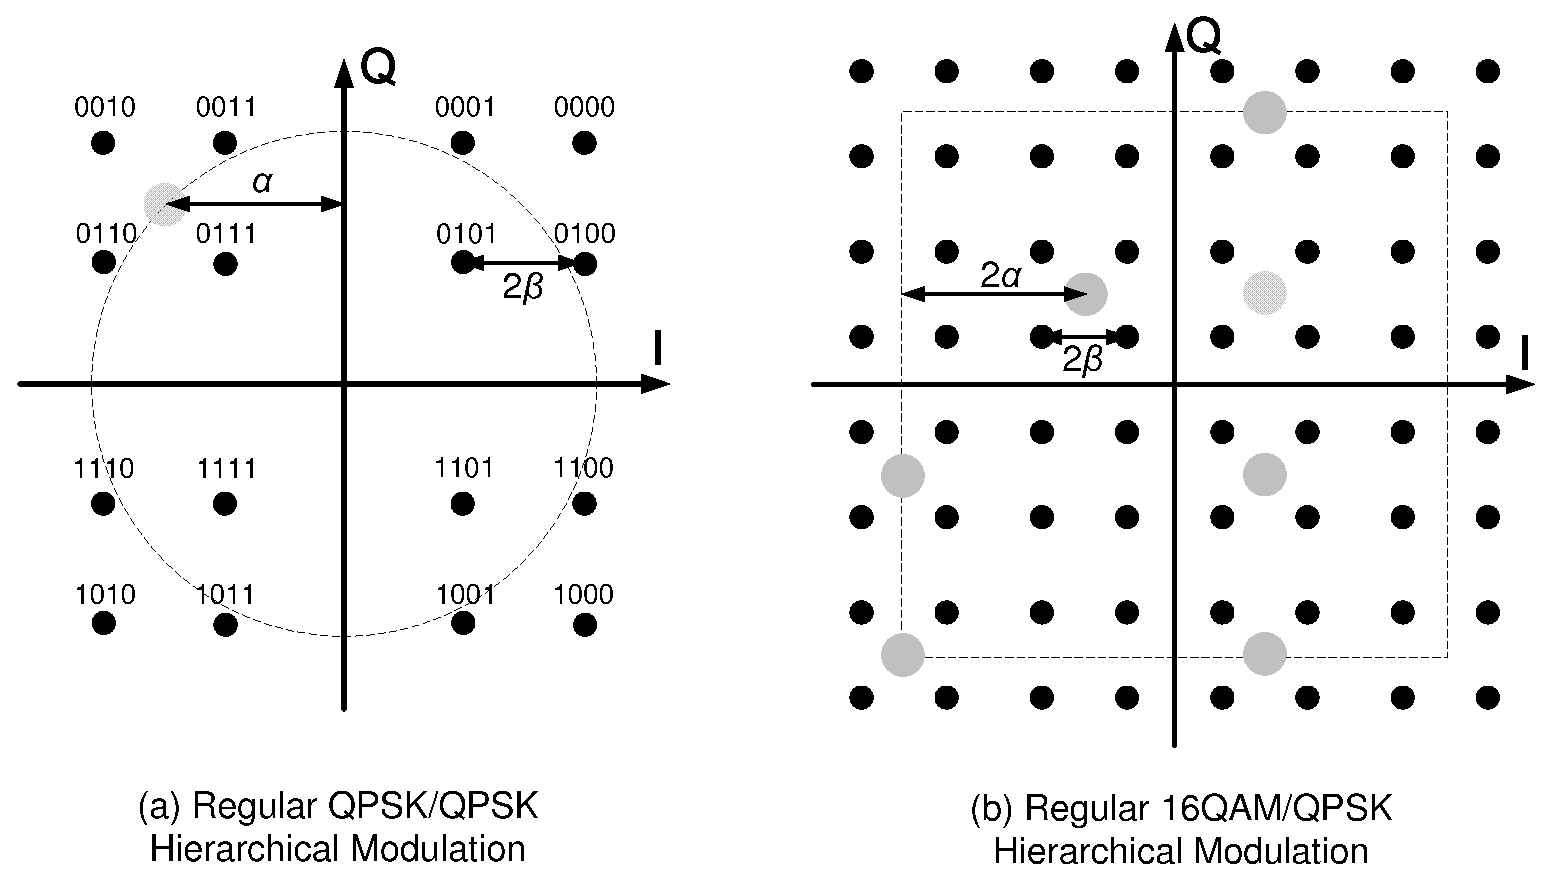
\includegraphics[width=3.0in, angle=0]{Regular_Hierarchical.eps}
\caption{Regular hierarchical modulation examples: the base layer
is QPSK/16QAM and the enhancement layer is
QPSK.}\label{regular_hierarchical} }
\end{figure}
\noindent Smaller minimum Euclid distance usually results in more
ambiguity and more demodulation errors.
And it is fixed regardless
the power-splitting ratio $\zeta$ between layers, which is defined
by
\begin{equation}
\begin{array}{rcl}
\zeta & = & \frac{P_{\rm E}}{P_{\rm B}}
\end{array}\label{power_ratio}
\end{equation}
\noindent with $\zeta < 1$ in most cases; Otherwise we think two
signal constellations exchanged layers in hierarchical signal
constellation. For QPSK/QPSK hierarchical modulation, the
power-splitting ratio is $\zeta_{\mbox{\tiny QPSK/QPSK}}=
\frac{\beta^{2}}{\alpha^2}$. For 16QAM/QPSK modulation,
$\zeta_{\mbox{\tiny 16QAM/QPSK}}= \frac{\beta^{2}}{4\alpha^2}$.
When $\zeta_{\mbox{\tiny QPSK/QPSK}}=\frac{1}{4}$, the QPSK/QPSK
modulation in Fig.~\ref{regular_hierarchical}(a) becomes
square-shaped 16QAM. In general, the enhancement-layer signal can
be taken as additional noise by base layer. At this time, most
existing conventional receivers can continue to demodulate
base-layer signals with no additional change but at a lower
signal-to-noise/interference ratio (SINR) $\hat{\gamma}$ defined
by
\begin{equation}
\begin{array}{rcccccl}
\hat{\gamma}& = & \frac{P_{\rm B}}{P_{\rm
E}+\sigma^2}&<&\gamma&=&\frac{P_{\rm B}}{\sigma^2}
\end{array}\label{SINR}
\end{equation}
\noindent with the background additive Gaussian white noise (AWGN)
power $\sigma^2$,  especially when $\zeta$ is small. On the other
hand, signals of both base layer and enhancement layer(s) can also
be demodulated by a advanced receiver. This is the strictly
backward compatibility of hierarchical modulation, which makes it
attractive for providing seamless upgrading with little change on
existing digital broadcast systems.

\subsection{Orthogonal Frequency-Division Multiplex and Peak-to-Average-Power Ratio}

An OFDM signal is the sum of $L$ independent modulated symbols
$\left\{s_{l}:\ 1\leq l\leq L\right\}$ mapped onto $L$ different
subcarriers with the frequency separation $\frac{1}{T}$, where $T$
is the symbol period with no additional overhead such as cyclic
prefix (CP) and zero prefix (ZP). At the transmitter side, the
discrete time-domain samples $\left\{x_{m}:\ 1\leq m\leq
L\right\}$ are the inverse fast Fourier transform (IFFT) of the
complex symbols $\left\{s_{l}:\ 1\leq l\leq L\right\}$:
\begin{equation}
\begin{array}{lcl}
x_{m}&=&\frac{1}{\sqrt{L}}\sum\limits_{l=0}^{L-1}s_{l}e^{j2\pi\frac{ml}{L}}
\end{array}.\label{OFDM}
\end{equation}
\noindent Before transmission, $x_{m}$ is usually extended by
attaching a CP or ZP. When CP is applied, the extended OFDM symbol
\begin{equation}
\begin{array}{rcl}
\tilde{x}_{n}&=&\Bigg\{ \begin{array}{ll}x_{n}&1\leq n\leq L\\
x_{n+L}&-L_{cp}+1\leq n\leq 0 \end{array}
\end{array}.
\end{equation}
\noindent The extended OFDM symbol then passes through
digital-to-analog converter and pulse-shaping filter before
up-converted to the carrier frequency. The PAPR of OFDM signal is
usually defined by
\begin{equation}
\begin{array}{rcl}
\xi&=&\frac{1 }{\mbox{E}\left\{\left|x_{m}\right|^2\right\}
}\max\limits_{m} \left|x_{m}\right|^{2}
\end{array},
\end{equation}
\noindent though in practice the PAPR of the analog signal
equivalent of $\left\{\tilde{x}_{n}:\ -L_{cp}+1\leq n\leq
L\right\}$ is more of interest.

\section{The Enhanced Hierarchical Modulation}

\begin{figure}
\center{
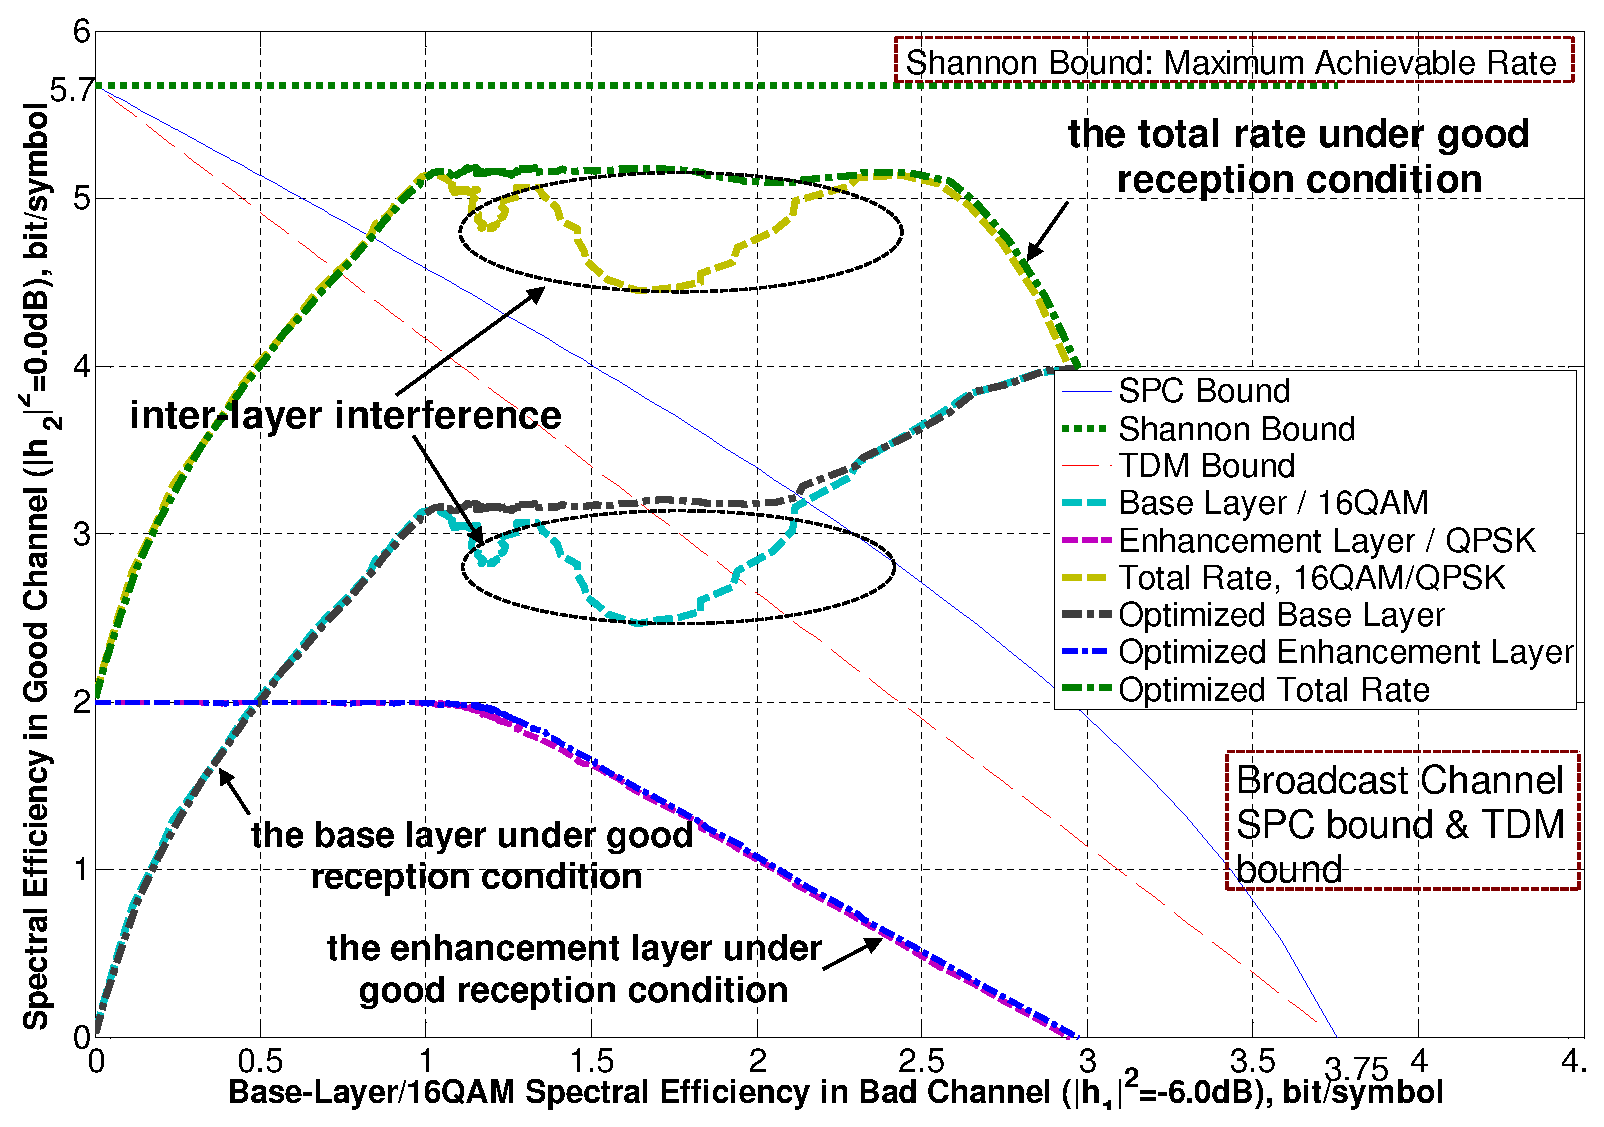
\includegraphics[width=3.0in, angle=0]{Capacity_100_025_16QAM.eps}
\caption{Achievable capacity of hierarchical modulations with
16QAM base layer and QPSK enhancement layer.}\label{Sum_Capacity}
}
\end{figure}

However, regular hierarchical modulation may seriously suffer from
ILI, which not only decreases the base-layer SINR from ${\gamma}$
to $\hat{\gamma}$ but also lowers the achievable spectral
efficiency. This is observed from Fig.~\ref{Sum_Capacity}. It is
well-known that the achievable throughput of a hierarchical
modulated signal essentially depends on the power distribution
profile of the signal~\cite{Unge82} in signal space instead of the
power-splitting ratio $\zeta$. This is similar to channel coding.
From a channel coding point of view, higher throughput is
achievable by the {\em i.i.d. Gaussian code} defined in coding
space, even though it may not be implementable from an engineering
standpoint~\cite{Cover72}. How to transmit a signal close to
Shannon channel capacity and implementable in a relatively easy
way is not only critical for the signal constellation design but
also every other component in a communication system.

The first approach is to optimize the signal constellation of
hierarchical modulation. This can help improve the spectral
efficiency of hierarchical modulation. There are many ways to do
it. The one we proposed is to optimally rotate the
enhancement-layer(s) of a signal constellation. For the QPSK/QPSK
hierarchical modulation shown in
Fig.~\ref{regular_hierarchical}(a), the QPSK signal constellation
of the enhancement layer is rotated in counter-clockwise by
$\theta$, $0\leq\theta\leq\frac{1}{4}\pi$, and resulted signal
constellation is shown in Fig. \ref{enhanced_hierarchical}(a). For
16QAM/QPSK, the regular and enhanced hierarchical modulations are
shown in Fig.~\ref{regular_hierarchical}(b) and Fig.
\ref{enhanced_hierarchical}(b), respectively.  As shown in
Fig.~\ref{Sum_Capacity}, with optimal rotation angle $\theta_{\rm
opt}$, most of the lost base-layer capacity can be recovered
without scarifying the throughput of enhancement layer(s) and the
achievable rate of QPSK-modulated enhancement layers is unchanged
before and after the rotation.
\begin{figure}
\center{
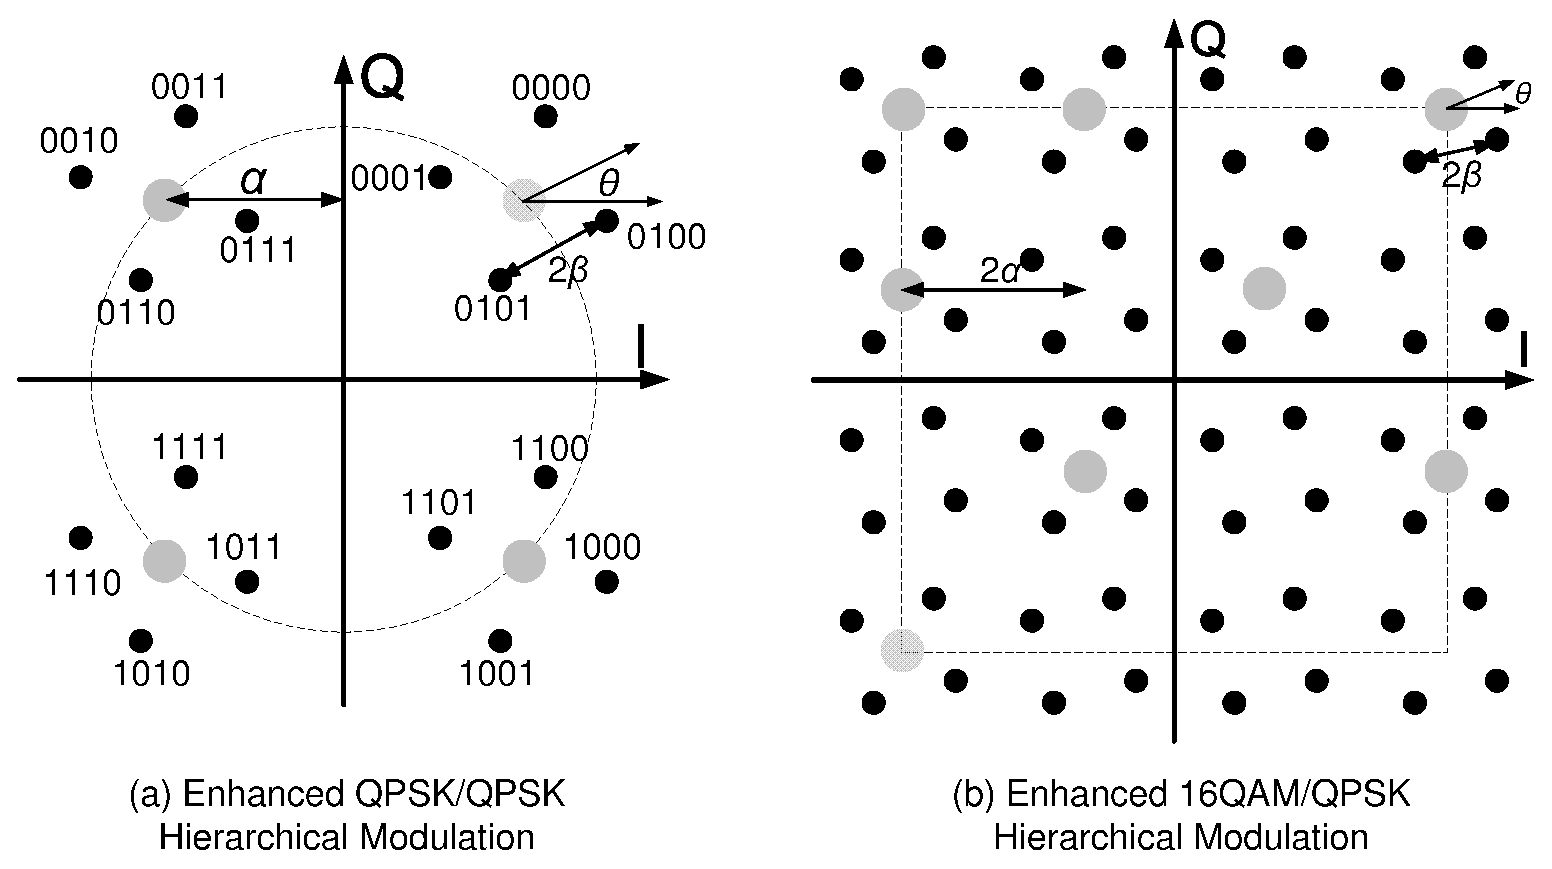
\includegraphics[width=3.0in, angle=0]{Enhanced_Hierarchical.eps}
\caption{Enhancing hierarchical modulation by
rotation.}\label{enhanced_hierarchical} }
\end{figure}

\section{Optimizing Hierarchical Modulation}

\subsection{Maximizing Achievable Rates~\label{Info_Theory}}

More three decades ago Cover showed that higher sum capacity is
achievable if messages for two users of different receptions are
superposited~\cite{Cover72}. Hierarchical modulation is one of the
practical implementations of superposition precoding (SPC) for
providing different rates and protections to users. In general,
the achievable rate of a $N$-ary modulated signal, of either
regular or hierarchical signal constellation, through AWGN channel
is given by~\cite{Unge82}
\begin{equation}
\begin{array}{lcl}
R&=&\log_{2}\left(N\right)-\\
&&\hspace{-0.20in}\frac{1}{N}\sum\limits_{i=0}^{N-1}\mbox{E}\left\{\log_{2}\left[\sum\limits_{j=0}^{N-1}e^{-\frac{\left|s_{j}+n-s_{i}\right|^2-\left|n\right|^2}{2\sigma^2}}\right]\right\}\
.
\end{array}\label{N_ary}
\end{equation}
\noindent This is the achievable rate when a receiver try to
decode the whole hierarchically modulated symbol. With
(\ref{N_ary}), the AWGN capacity of regular QPSK and 16QAM can be
plotted in Fig \ref{capacity_16QAM}. Though the rate in
(\ref{N_ary}) is achievable by users with advanced receiver, it is
more than achievable for a user with a conventional receiver which
usually detects the base-layer signals only. The achievable rate
of either base layer or enhancement layer is lower than the total
rate in (\ref{N_ary}). Following the concept of the successive
interference cancellation, the achievable rate, also termed {\em
equivalent capacity}, for a receiver decoding up to $l$ layers of
a hierarchical modulated symbol is~\cite{Huber94}
\begin{equation}
\begin{array}{rcccl}
\tilde{R}_{l}&=&\sum\limits_{i=0}^{l-1}R_{i}& = &
R-\sum\limits_{j=l}^{L}{R}_{j}
\end{array}.\label{R_equiv}
\end{equation}
\noindent To illustrate this, let's take the regular 16QAM as an
example since a regular 16QAM can be take as a special case of
QPSK/QPSK hierarchical modulation with $\zeta_{\mbox{\tiny
QPSK/QPSK}}=\frac{1}{4}$. This means the achievable rate of the
enhancement layer is the same as the regular QPSK capacity but the
achievable rate of the QPSK base layer becomes
\begin{equation}\hspace{-0.2in}
\begin{array}{rl}
{\rm R}_{\mbox{\tiny QPSK/QPSK}}^{\rm B}\left(\gamma,\
\frac{1}{5}\right)&\hspace{-0.08in}=\ {\rm R}_{\mbox{\tiny
QPSK/QPSK}}\left(\gamma,\
\frac{1}{5}\right)-{\rm R}_{\mbox{\tiny QPSK}} \left(\frac{1}{5}\gamma\right)\\
&\hspace{-0.08in}=\ {\rm R}_{\mbox{\tiny
16QAM}}\left(\gamma\right)-{\rm R}_{\mbox{\tiny
QPSK}}\left(\frac{1}{5}\gamma\right)\ .
\end{array}\label{R_16QAM_B1}
\end{equation}
\noindent They are plotted in Fig \ref{capacity_16QAM}. Due to the
ILI from the QPSK-modulated enhancement layer, the actual
throughput of the QPSK base layer ${\rm R}_{\mbox{\tiny
QPSK/QPSK}}^{\rm B}\left(\gamma,\ \frac{1}{5} \right)$ is lower
than the corresponding QPSK rate ${\rm R}_{\mbox{\tiny
QPSK}}\left(\frac{4}{5}\gamma\right)$, i.e.,
\begin{equation}
\begin{array}{rcl}
{\rm R}_{\mbox{\tiny QPSK/QPSK}}^{\rm B}\left(\gamma,\ \frac{1}{5}
\right)&\leq&{\rm R}_{\mbox{\tiny QPSK}}
\left(\frac{4}{5}\gamma\right)
\end{array}.\label{R_16QAM_B2}
\end{equation}
\begin{figure}
\center{
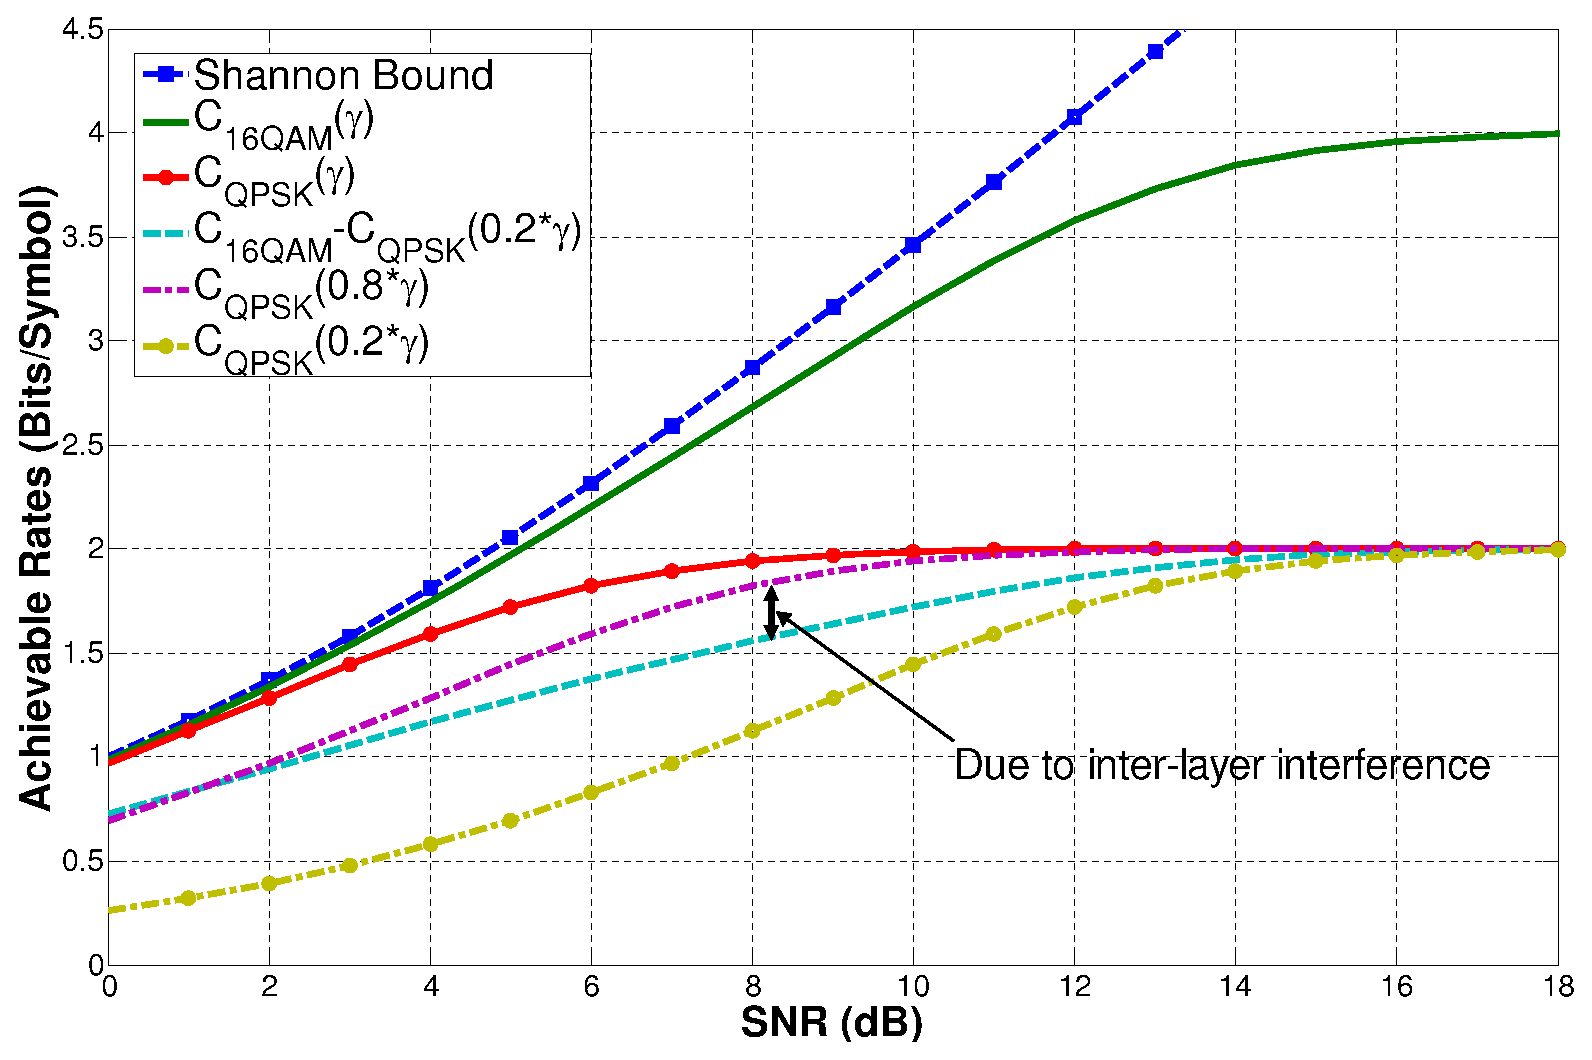
\includegraphics[width=3.0in, angle=0]{Capacity_16QAM.eps}
\caption{Achievable rates of regular 16QAM modulation: a
hierarchical modulation perspective.}\label{capacity_16QAM} }
\end{figure}
\noindent In Fig \ref{capacity_16QAM}, it shows that the
degradation of the base-layer capacity can be up to around
$\Delta=0.56$ bits/symbol, which is about $14\%$ of the maximum
total achievable rate $2$ bits/symbol for the QPSK base-layer.
This kind of degradation can be further illustrated in
Fig.~\ref{capacity_rotating}, where the hierarchical modulation is
16QAM/QPSK-modulated. In Fig.~\ref{capacity_rotating}, the total
SNR is fixed at $\frac{P}{\sigma^2}=20\mbox{dB}$ but the power of
the 16QAM sublayer is changed from $0\%$ to $100\%$ of the total
power $P$. The achievable rates of each layer and the whole signal
constellation are plotted in Fig.~\ref{capacity_rotating}. One of
the interesting things shown in Fig. \ref{capacity_rotating} is
the equivalent capacity of the 16QAM base layer changes
periodically instead of monotonically with increase the power
ratio of the base layer. The good things in Fig.
\ref{capacity_rotating} is this kind of capacity loss can be
recovered by optimally rotating the enhancement layer. This is one
of the advantages of the proposed enhanced hierarchical
modulations.
\begin{figure}
\center{
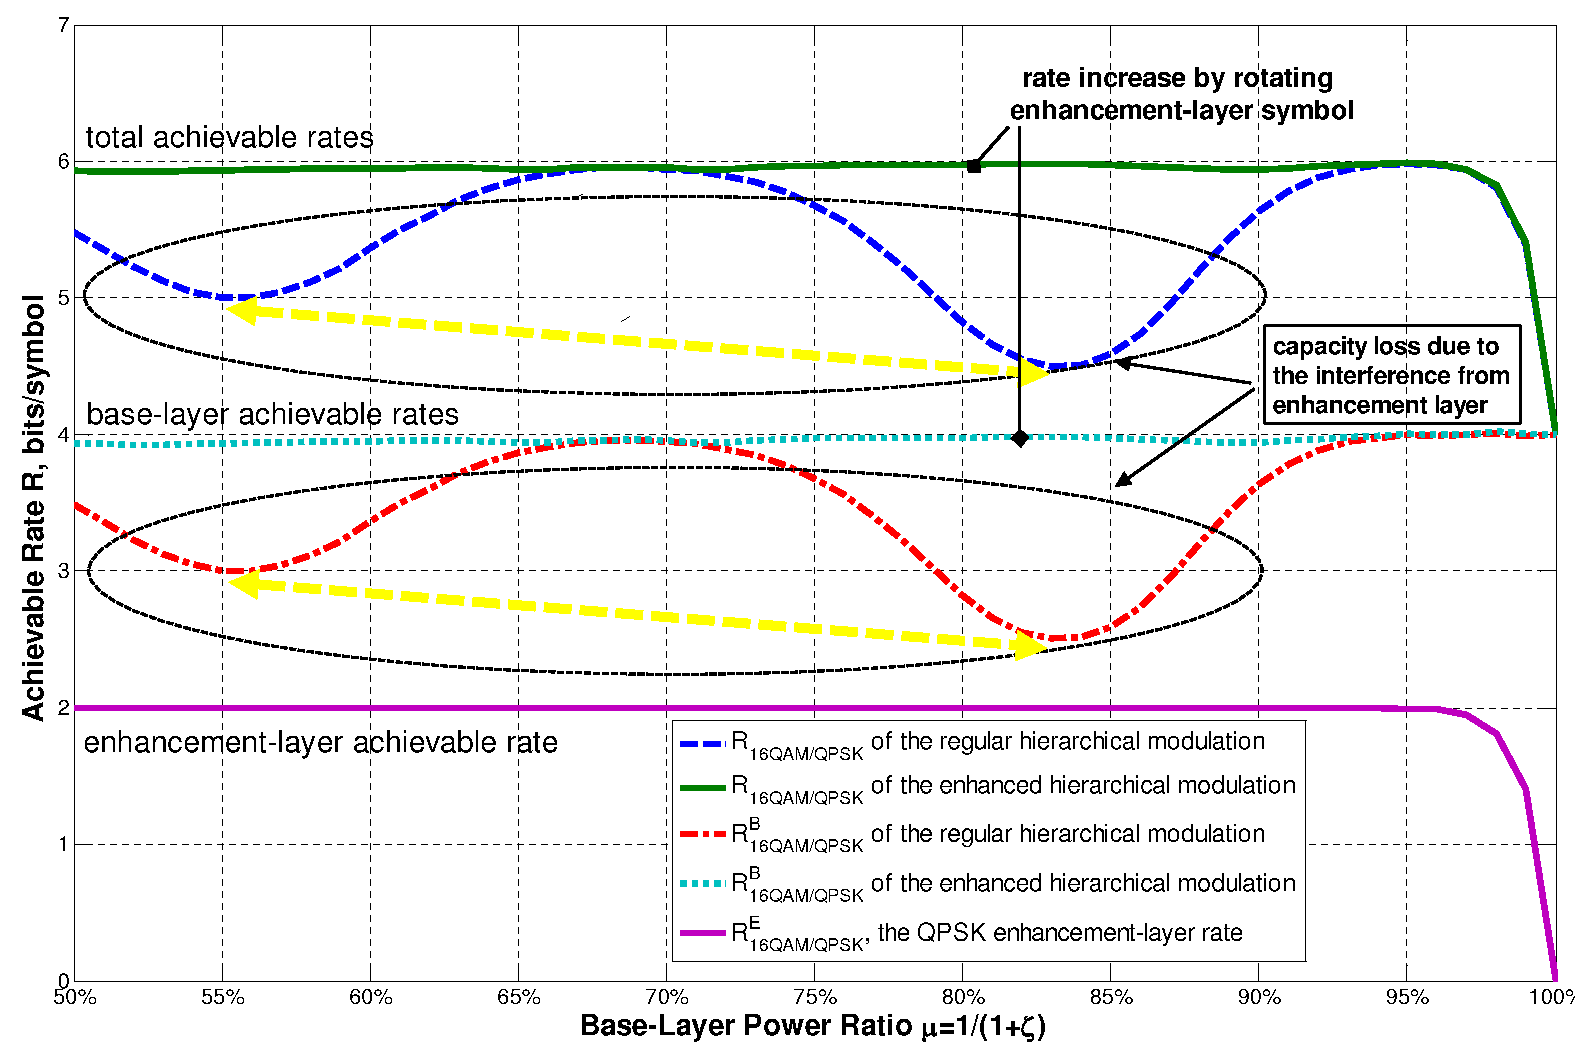
\includegraphics[width=3.0in, angle=0]{Capacity_power_splitting.eps}
\caption{Achievable rates of 16QAM/QPSK hierarchical modulation
with different power splitting and
$\frac{P}{\sigma^2}=20$dB.}\label{capacity_rotating} }
\end{figure}

\subsection{Maximizing Modulation Efficiency}

Besides the above information-theoretical point of view on
hierarchical modulation, it is also interesting to understand
hierarchical modulation from a practical signal-processing
perspective. At this time, the performance of hierarchical
modulation will be evaluated through actual implementations, where
demodulation BER is one of the major concerns. In general, it is
difficult to give a simple closed-form BER expression for
hierarchical signal constellation, which also depends on receiver
design. The BER of square-shaped $M$-QAM constellation and a
hierarchical QAM constellation for maximum likelihood (ML)
demodulator can be computed by using recursive
algorithms~\cite{Vitt03}. It is known that the BER expression for
QPSK is
\begin{equation}
\begin{array}{rcl}
{\rm P}_{e,\mbox{\tiny QPSK}}\left(\gamma\right)&=&{\rm
Q}\left(\sqrt{\frac{\gamma}{2}}\right)
\end{array},\label{BER_QPSK}
\end{equation}
\noindent where ${\rm Q}\left(x\right)=\frac{1}{2}{\rm
erfc}\left(\frac{x}{\sqrt{2}}\right)$ denotes the $\rm
Q$-function.
\begin{figure} \center{
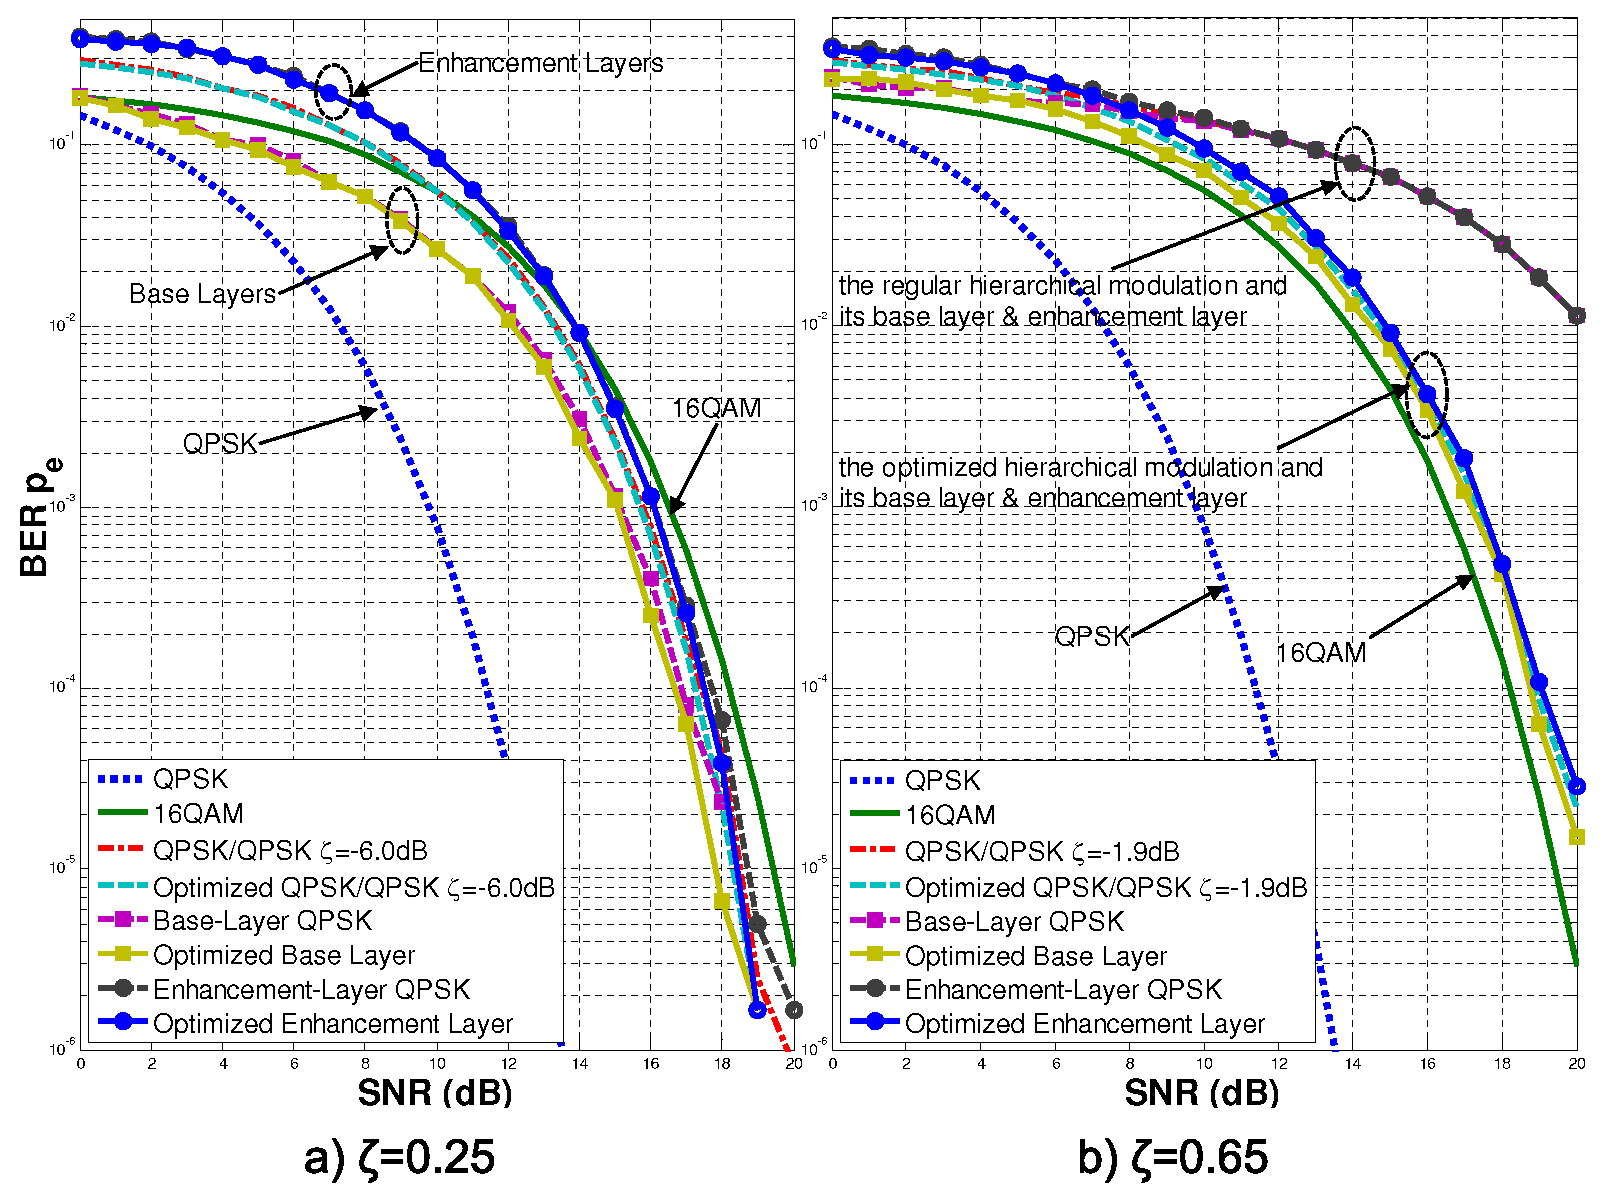
\includegraphics[width=3.20in, angle=0]{BER_Hierarchical.eps}
\caption{Bit-error rate of uncoded QPSK/QPSK hierarchical
modulations using maximum likelihood demodulation . } \label{BER}}
\end{figure}
From a signal processing standpoint, the BER and capacity
degradation may happen when there is a change in noise and/or
interference distribution, even though the received SNR $\gamma$
is the same. For example, the BER performance of regular QPSK/QPSK
becomes deteriorated in Fig. \ref{BER} when increase
$\zeta_{\mbox{\tiny QPSK/QPSK}}$. But, if we optimally rotate the
enhancement-layer signal constellation, the performance loss can
be recovered. This kind of recovery is more significant with large
$\zeta$. There are many ways for quantifying and understanding
this kind of BER performance loss due to interference and receiver
design. One approach for capturing this kind of degradation is to
calculate the effective signal-to-noise ratio (ESNR) on the
receiver output, which is defined by
\begin{equation}
\begin{array}{rcl}
\tilde{\gamma}\left(\gamma\right)&\equiv&\Psi^{-1}\left(p_{e}(\gamma)\right)
\end{array},\label{eff_SNR}
\end{equation}
\noindent where $p_{e}(\gamma)$ is the demodulation BER of the
signal with SNR $\gamma$, and $\Psi^{-1}\left(\ast\right)$ denotes
the inverse function of $\Psi\left(\cdot\right)$, the demodulation
error probability function with no ILI. For example, the ESNR for
the QPSK-modulated base layer or enhancement layer of any
hierarchical modulation can be calculated by
\begin{equation}
\begin{array}{rcl}
\tilde{\gamma}_{\mbox{\tiny QPSK/QPSK}}&=&2\left[{\rm
Q}^{-1}\left(p_{e}(\gamma)\right)\right]^2
\end{array}.\label{eff_SNR_QPSK}
\end{equation}
\noindent More specifically, the ESNR for the base layer of
regular QPSK/QPSK hierarchical modulation with ML demodulator is
given by
\begin{equation}\hspace{-0.225in}
\begin{array}{l}
\tilde{\gamma}_{\mbox{\tiny QPSK/QPSK}}^{\rm
B}(\gamma)=2\left[{\rm Q}^{-1}\left(\frac{{\rm
Q}((1-\sqrt{\zeta})\gamma)+{\rm
Q}((1+\sqrt{\zeta})\gamma)}{2}\right)\right]^2.
\end{array}\label{eff_SNR_QPSK_QPSK}
\end{equation}
\noindent By normalizing ESNR by $\gamma$, we can obtain
hierarchical modulation efficiency (ME) $\eta$ by
\begin{equation}
\begin{array}{rcccl}
\eta\left(\gamma\right)&=&\frac{\tilde{\gamma}}{\gamma}&=&\frac{1}{\gamma}\Psi^{-1}\left(p_{e}(\gamma)\right)
\end{array}.\label{mod_eff}
\end{equation}
\noindent With no interference, $\eta\left(\gamma\right)=1$;
otherwise, $\eta\left(\gamma\right)<1$. $\eta$ is also the measure
of inter-layer resistance for hierarchical modulation. Higher ME
is, stronger interference-resistance the signal has. As an
example, the ME of QPSK/QPSK hierarchical modulation are plotted
in Fig. \ref{modulation_efficiency}. We can see the enhanced
hierarchical modulation has higher ME than the regular modulation.
The difference is more obvious when $\zeta$ becomes large. This
means enhanced hierarchical modulation has stronger inter-layer
interference resistance than regular hierarchical modulation.
\begin{figure}
\center{
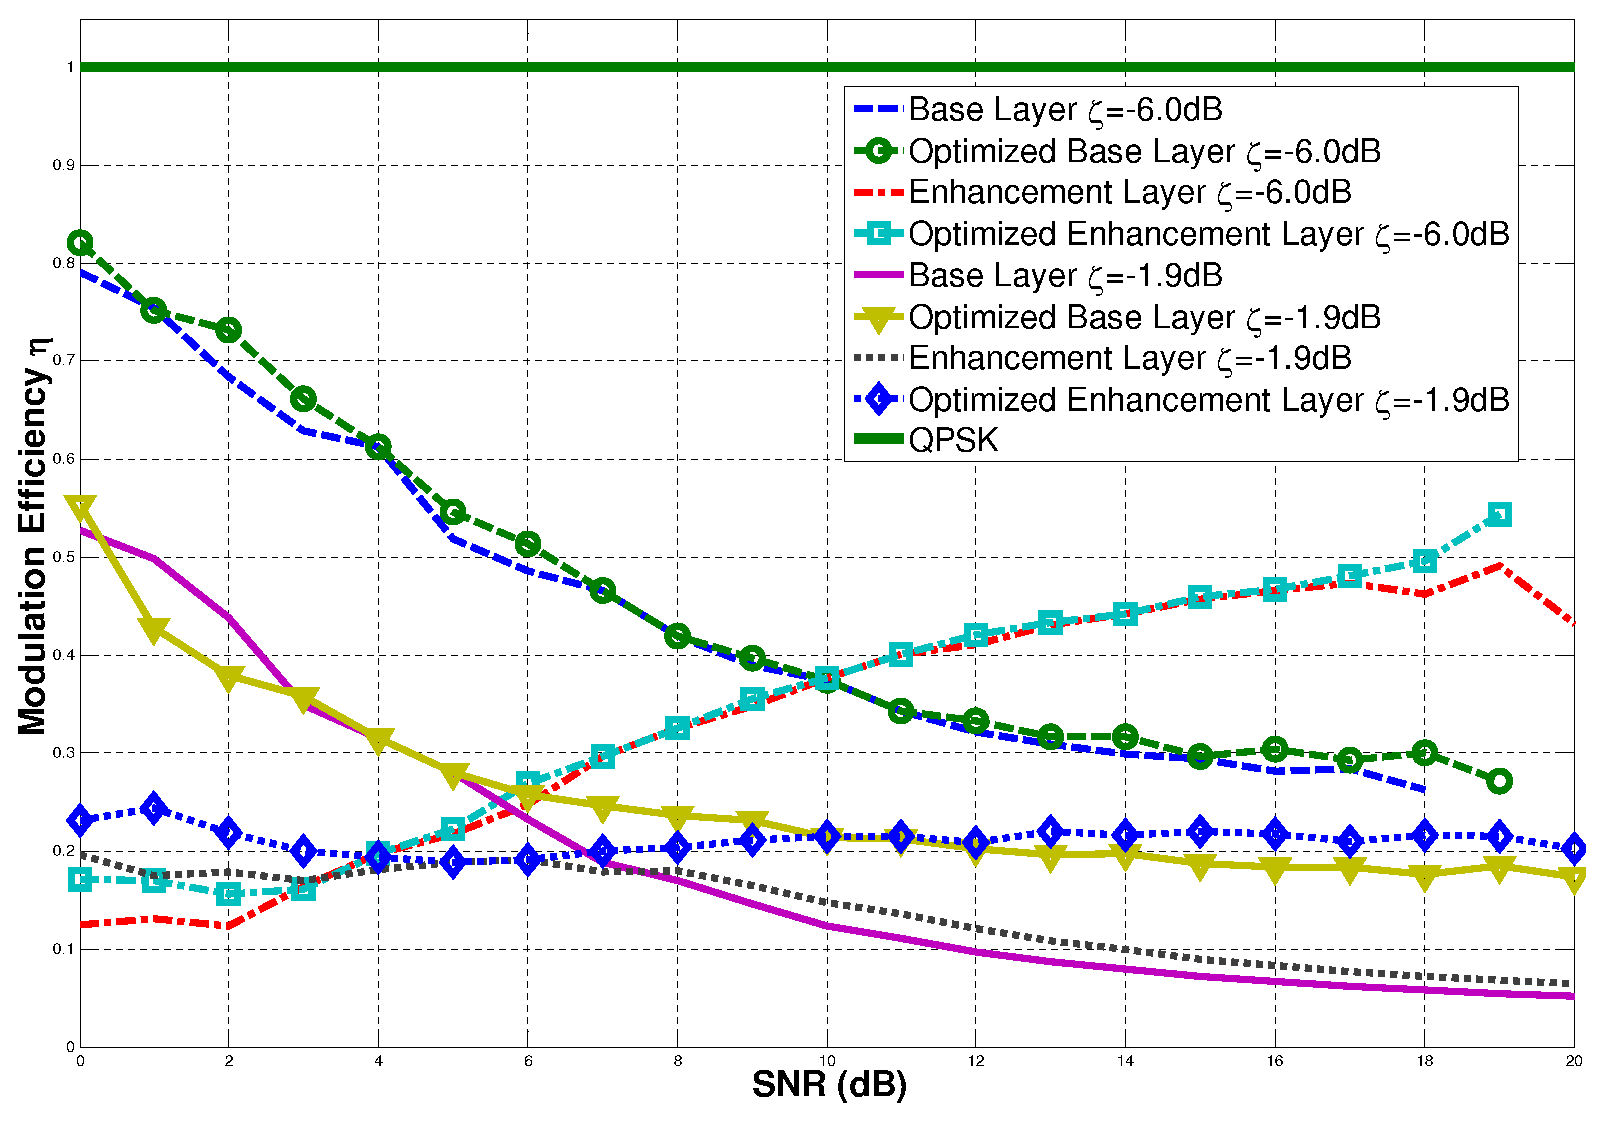
\includegraphics[width=3.0in, angle=0]{Modulation_Efficiency.eps}
\caption{Hierarchical modulation efficiency of QPSK/QPSK
hierarchical modulation using maximum likelihood
demodulation.}\label{modulation_efficiency} }
\end{figure}

The asymptotic modulation efficiency (AME) $\eta_{\infty}$ is
given by
\begin{equation}
\begin{array}{rcccl}
\eta_{\infty}&=&\lim\limits_{\gamma\rightarrow\infty}\eta\left(\gamma\right)&=&\lim\limits_{\sigma\rightarrow0}\frac{\sigma^2}{P}\Psi^{-1}\left(p_{e}\right)
\end{array}.\label{asy_mod_eff}
\end{equation}
\noindent For the example in (\ref{eff_SNR_QPSK_QPSK}), the AME
can be calculated by
\begin{equation}\hspace{-0.225in}
\begin{array}{rcl}
\eta_{\infty}&=&\lim\limits_{\gamma\rightarrow\infty}\frac{2\left[{\rm
Q}^{-1}\left(\frac{{\rm Q}((1-\sqrt{\zeta})\gamma)+{\rm
Q}((1+\sqrt{\zeta})\gamma)}{2}\right)\right]^2}{\gamma}.
\end{array}\label{asy_eff_SNR_QPSK_QPSK}
\end{equation}
\noindent From (\ref{asy_mod_eff}) and
(\ref{asy_eff_SNR_QPSK_QPSK}), it shows that AME basically shows
how fast ESNR is approaching SNR when $\gamma\rightarrow\infty$.
This can be expressed by
\begin{equation}
\begin{array}{rcl}
\eta_{\infty}&=&\frac{\partial\eta\left(\gamma\right)}{\partial\gamma}|_{\gamma=\infty}
\end{array}.\label{asy_mod_eff2}
\end{equation}
\noindent The AME for QPSK/QPSK hierarchical modulation can also
be found in Fig.~\ref{modulation_efficiency}, in which they are
the points approached when SNR becomes larger and larger.

\subsection{Minimizing Peak-to-Average-Power Ratio}

The RSSPA model of HPA is defined by
\begin{equation}
\begin{array}{rcl}
v_{\rm o}&=&\frac{v_{\rm i}}{\left[1+\left(\frac{|v_{\rm
i}|}{V_{\rm s}}\right)^{2p}\right]^{\frac{1}{2p}}}
\end{array},\label{RSSPA}
\end{equation}
\noindent where $v_{\rm i}$ and $v_{\rm o}$ respectively denote
the complex input and output signals, $V_{\rm s}$ denotes the
output saturation voltage level with $P_{\rm s}=\left|V_{\rm
s}\right|^2$ and $p$ denotes the knee factor, which controls the
smoothness of HPA characteristic.



\section{Conclusions}
In this paper, two schemes for enhancing hierarchical modulations
are presented for higher throughput and less error rate. One
approach is to optimize the signal constellation and the other one
is to optimize the bits-to-symbol mapping. The rationales as well
as the performance of the proposed approaches are analyzed. They
can be used for helping upgrade and design BCMCS systems with
minimum complexity increase. Some of them is adopted in the 3.5G
standard UMB by 3GPP2. \small
\bibliographystyle{unsrt}
\bibliography{Hierarchical_Modulation}
\end{document}
